\section{Vorgehensmodell zur Umsetzung für Cloud Computing}
\label{VgmVorgehensmodell}
%=============================
\begin{flushright}{\slshape    
    [With legacy systems] the cost is getting higher because maintenance is getting more expensive, [then] maybe you should think of modernization}
    --- unbekannt \cite{profperLeg}
\end{flushright}

Die Entwicklung, der Betrieb, die Betreuung und die stetige Weiterentwicklung durch neue Anforderungen von  Software im Unternehmen erfordert  mehr Expert:innenwissen als früher. Ursache dafür ist auch der immer größer werdende Anteil künstlicher Intelligenz in Applikationen. Es wird Hardware benötigt. Ebenso weitere physischer Computerressourcen für Fallback-Szenarien, die auf die Gewährleistung von (IT-)Compliance einzahlen.
\\\\
Repräsentative und auswertbare Studien bereits umgesetzter Modernisierungen größerer Unternehmen finden sich in der Literatur nur wenige. Etwaige Gründe dafür könnten sein, dass diverse erfolgreiche Lösungen aufgrund des Konkurrenzdenkens und resultierenden Marktvorteil nicht veröffentlicht werden.  Obwohl immer mehr Unternehmen die Bedeutung und die Vorteile von signifikant besser wartbarer und skalierbarer Software erkennen, führen sie keine Modernisierungsmaßnahmen durch. Eine mögliche Erklärung dafür kann an dem mangelnden Fachpersonal liegen.  \\\\

Trotz einer gut definierten Enterprise-Architektur und unmissverständlich dokumentierten Sourcecode ( \nameref{refactoring}) einer Legacy-Software, begegnen dem (IT-)Personal viele Hürden. Der Weg der Legacy Software bis hin zur „modernen Software“ muss klar definiert, strukturiert und deterministisch sein. \\\\
Die Software-Modernisierung einer Legacy ist keineswegs trivial. Zahlreiche Herausforderungen, die nicht nur Geld kosten, erschweren den Weg von der Legacy zur modernen Software. Wie kann die zukünftige Software qualitativ verbessert werden?  Was  gilt überhaupt zu beachten? Welche Anforderungen galten bisher? Wie soll die Ziellandschaft aussehen? Eine ausgeklügelte Strategie kann für den langfristigen  Erfolg und Erhalt der Software sorgen.  Die Unternehmen benötigen eine Roadmap/ ein Vorgehensmodell. Es soll alle notwendige Schritte definieren, alle Fragestellungen kategorisch zusammenfassen und die Unternehmen in jedem Schritt der Modernisierungsmaßnahme unterstützen. 
\\\\
In der Literatur gibt es diverse Vorgehensmodelle zur Umsetzung von Modernisierungsmaßnahmen. Die Vielfalt dieser liegt unter anderem in den unterschiedlichen Anforderungen, verfügbaren Ressourcen, dem Risiko-Management, der zu modernisierenden Software und auch mit der mittel- bis langfristigen Unternehmensstrategie. \cite{10.1145/2818567.2818579}

\subsection{ARTIST EU} 
Ein Modell-getriebener Ansatz Europäischen Union nennt sich\textit{ \ac{ARTIST}}.\cite{artistEU} Die \acs{ARTIST} Methoden und  \acs{ARTIST} Frameworks, sollen die Entwickler und Entwicklerinnen in jedem Schritt der Migration- und Modernisierungsmaßnahme unterstützen. Dabei fasst es bereits Best-practises zusammen\cite{menychtas2014software}. In Teilen verwendet \acs{ARTIST} die \ac{SMART} die in der Pre-Migration-Phase stattfindet. \\\\
 \acs{SMART} wird unter anderem auch für die Analyse der Legacy verwendet, um festzustellen, ob beispielsweise ihre Funktionalität oder Teile davon als Services (\acs{SOA}) bereitgestellt werden können. Die Interaktion eines Legacy-Systems innerhalb einer \acs{SOA}, wie beispielsweise einer Web-Services-Architektur, ist manchmal relativ einfach – was wiederum sehr attraktiv für die Unternehmen ist. Web-Service-Schnittstellen sind so eingerichtet, dass sie SOAP-Nachrichten empfangen und analysiert werden, wodurch der entsprechende Dienst direkt aufgerufen werden kann. Zahlreiche neue Entwicklungsumgebungen bieten Tools, die diesen Prozess unterstützen. Unternehmen setzen eben diese Umgebungen  ein, um ihre Geschäftsprozesse der Welt zugänglich zu machen.\cite{lewis2005service} 
 
 
 
 
 
\subsection{Roadmap}
Das Vorgehensmodell zur Modernisierung einer Legacy von S. Jain und I. Chana \cite{ccRoadmap} wird  nun betrachtet. Einen groben Überblick bietet folgende Abbildung, die die wesentlichen Hauptkomponenten des Vorgehensmodells darstellt.


\begin{figure}[h] 
  \centering
  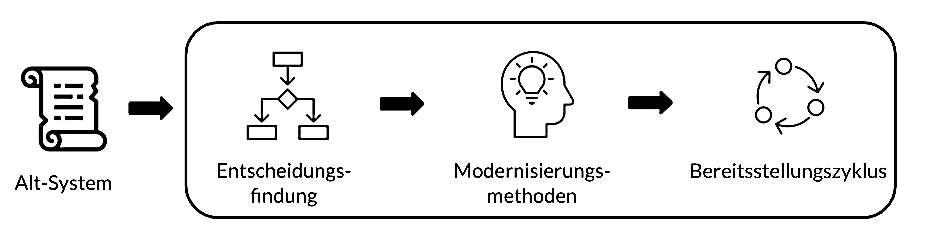
\includegraphics[width=0.7\textwidth]{Chapters/Vorgehensmodell/images/ccvorgehensmodell.png}
  \caption{Vorgehensmodell zur Umsetzung einer Modernisierungsmaßnahme für Cloud Computing. \cite{ccRoadmap}}
  \label{fig:picCCRoadmap}
\end{figure}

Erstens, das Entscheidungsmodul. Wieder rum besteht aus drei Hauptkomponenten, die im Wesentlich zur Bewertung des Alt- und Zielsystem eine Grundlage bilden.\\
Zweitens, das Modul für Modernisierungsmethoden. Hier stehen uns vier Schlüsselmethoden zur Auswahl, um die Modernisierungsmaßnahme mit einem geeigneten Ansatz und einer geeigneten Implementierung fortzusetzen.
Drittens, der Bereitstellungszyklus. Er beschreibt nach den ersten beiden Modulen einen permanenten Zyklus, bestehend aus vier zusammenfassenden Schritten.
\\\\
\addsec{Entscheidungsfindung}
Das erste Modul kann im Weiteren in drei weitere Module unterteilt werden.
\begin{description}   
 \item [Beurteilung des Altsystems] \hfill \\
Die Bestimmung der Komplexität für die Modernisierungsmaßnahme ist ein Hauptfaktor  um den Aufwand und die Kosten für das Projekt bestimmen zu können.  Dabei müssen die unterschiedlichen Schichten der Software, oder der IT-Infrastruktur betrachtet werden. Verglichen mit dem OSI-7-Layer Modell müssen die sieben Schichten Physical-, Data Link-, Network-, Transport-, Session-, Presentation-, Session- und Application-Layer untersucht werden \cite{briscoe2000understanding}.  Hier sollte bestimmt werden, in welchen Schichten beispielsweise die Business Logik liegt und mit welchen anderen Layern sie korrespondiert. Die Komponenten, die in das Cloud-System migriert werden sollen, beeinflussen somit die Skalierbarkeit der Applikationen in. 
 \item [Beurteilung (bisherige) Servicequalität] \hfill \\
Ebenfalls muss die bisherige Qualität analysiert werden. Was war bisher schlecht und was könnte  im Zuge der Modernisierung besser gemacht. Aus technischer sowie auch fachlicher Sicht. Konkret bedeutet das, ob man beispielsweise durch ein Redesign des Prozesses größere qualitative als auch quantitative Erfolge erzielen kann. Das könnten beispielsweise verkürzte Arbeitswege sein.
 \item [Bestimmung von Zielen] \hfill \\
 Aus den bisherigen Betrachtungen sollten nun die Ziele bestimmt werden. Das könnte auf allgemeinen Ebene z.B. sein: Ein besseres Management der Plattform, der Infrastruktur oder der Services. In Hinblick auf den Code können eine bessere Wartbarkeit, eine bessere Codequalität und quantitativ verringerte Komplexität von Funktion ebenso weitere Ziele sein. 
 \end{description}
 
\addsec{Medornisierungsmethoden}
S. Jain et al. stellen in ihrem Vorgehensmodell folgende vier Schlüsselmethoden vor
\begin{description}   
 \item [Ersetzung] \hfill \\
 Denkbar ist eine komplette Ersetzung von Software-Komponenten durch bereits existierende Software von Drittanbietern. COTS \cite{cots} gehen mit einem geringeren Risiko einher, da die Software bereits etabliert und getestet ist. Oftmals ist aber kein direkter Kauf mehr möglich, da viele Drittanbieter ihre Lösungen über diverse Lizenzmodelle anbieten. Das führt zu dem Nachteil, dass ein Unternehmen mittel- bis langfristig in hohem Maße von dem Anbieter abhängig sind. \\Ebenfalls kommt dieser Ansatz nicht infrage, sofern die bewertete Business-Logik sehr an die Bedürfnisse der Unternehmen angepasst wurde und damit nicht hundertprozentig mehr mit COTS ersetzbar ist.
 
 \item [Black Box Wrapping] \hfill \\
 In diesem Ansatz wird ein neues Interface lediglich an alte Komponenten der Legacy in der Cloud-Umgebung angebunden. Umsetzbar ist dieser Ansatz nur dann, wenn der Code der Legacy in einem gut-verwertbaren Zustand ist (vgl. \nameref{refactoring}). Ebenfalls beinhaltet dieser Ansatz eine sukzessive Anpassung der noch bestehenden Altsoftware im neuen System.
 \item [Reengineering/Redevelopment] \hfill \\
 Übergreifend mit dem Begriff Software-Engineering wird hier verwendet. Dieser Ansatz stellt somit eine komplette Neuentwicklung des Systems dar, mit teilweise Wiederverwendung oder Verbesserungen des alten Codes.
 \item [Migration] \hfill \\
\textit{} Das komplette System mit Kernfunktionalität wird in eine neue Umgebung repliziert, mittels unterschiedlicher Migrationsstrategien. So können auch Altsysteme bestehend und ohne Veränderung auf einer virtuellen Umgebung kurz- bis mittelfristig geparkt werden. Anschließend kann eine sukzessive Anpassung der Software erfolgen. An dieser Stelle erwähnenswert sind die Arten, wie spätere Dienste oder Applikationen in der Cloud angeboten und dargestellt werden können. Konkret handelt es sich hierbei um \ac{IaaS}, \ac{PaaS} und \ac{SaaS}. Diese Begriffe werden in Kapitel \textit{\ref{VgmAsAService} \nameref{VgmAsAService}} näher behandelt.
\end{description}   


\addsec{Bereitstellungszyklus}

\begin{figure}[h] 
  \centering
  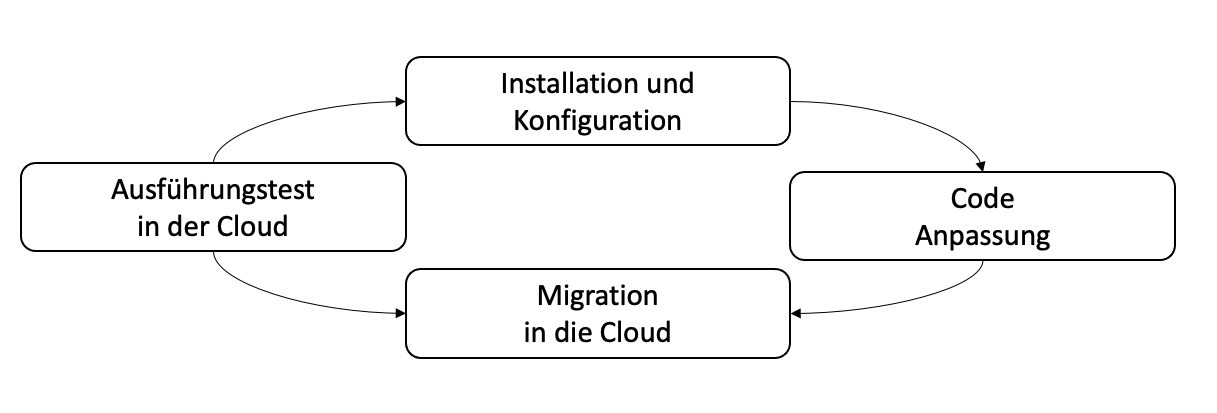
\includegraphics[width=0.8\textwidth]{Chapters/Vorgehensmodell/images/Bereitstellungszyklus.png}
  \caption{Bereitstellungszyklus im Vorgehensmodell \cite{ccRoadmap}}
  \label{fig:Bereitstellungszyklus}
\end{figure}
Nach der Selektion des geeigneten Ansatzes wird inkrementell mit der Implementierung begonnen, um die Modifikationen schrittweise mit den betroffenen Bestandteilen abzubilden. Mit der ersten Phase beginnend, kommt die Einrichtung und Einstellung der nötigen Tools für die Migration.  Einzelne Code-Segmente werden in den zirkulierenden Phasen priorisiert angepasst.
Es muss stets ein Fallback-Szenario vorhanden sein, bevor Änderungen am Quellcode durchgeführt werden. Hier kann ein Replikat der funktionierenden Alt-Version verwendet. 
Die modifizierte Komponente wird dann in der Cloud mit ausgewählten Servicemodellen (vgl. \textit{\ref{VgmAsAService} \nameref{VgmAsAService}}) und den jeweiligen Bereitstellungskonfigurationen gehostet. Abschließend findet in jedem Zyklus ein vollumfänglicher Test der Funktionalität innerhalb der Cloud statt, damit das System auch stets funktionsfähig bleibt und korrekt arbeitet.
 

